\documentclass[thesis.tex]{subfiles}

\begin{document}
\emph{Ab initio} structure calculations of many-fermion systems such as those in nuclear and electronic structure aim to describe emergent phenomena from the constituent particles subject to the underlying microscopic Hamiltonian.  This amounts to finding the solution to the many-body Schr\"{o}dinger equation.  However, a calculation of the exact solution needs to account for all possible correlations among the particles and thus scales factorially.  This motivates the need for approximations to the exact solution that account for the most important correlations.  This chapter first establishes the formalism necessary to define the many-body problem then illustrates several successive approximations to its solution.  Because the type of fermions and the underlying Hamiltonian can be kept generic until specific systems are considered, the formalism and many-body methods can be kept generic as well.


\section{Independent-Particle Model}
The nonrelativistic $A$-body quantum problem begins with the Schr\"{o}dinger equation,
\begin{equation} \label{eq:schrodinger}
  \Ham\Psi_{\nu}\left(\mathbf{r}_{1},\cdots,\mathbf{r}_{A}\right) = E_{\nu}\Psi_{\nu}\left(\mathbf{r}_{1},\cdots,\mathbf{r}_{A}\right),
\end{equation}
for the correlated wave function $\Psi_{\nu}\left(\mathbf{r}_{1},\cdots,\mathbf{r}_{A}\right)$ and the corresponding energy $E_{\nu}$.  The Hamiltonian can be written generically as a sum of $k$-body pieces which, in principle, can contain up to $A$-body interactions,
\begin{align} \label{eq:hamiltonian}
  \Ham &= \HamB{1} + \HamB{2} + \HamB{3} + \cdots \notag \\
  &= \sum^{A}_{\mathclap{i}}\HamB{1}\left(\mathbf{r}_{i}\right) + \sum^{A}_{\mathclap{i<j}}\HamB{2}\left(\mathbf{r}_{i},\mathbf{r}_{j}\right) + \sum^{A}_{\mathclap{i<j<k}}\HamB{3}\left(\mathbf{r}_{i},\mathbf{r}_{j},\mathbf{r}_{k}\right) + \cdots.
\end{align}
Regardless of the system, the one-body term contains the kinetic energy operator $\frac{-\hbar^{2}}{2m}\nabla^{2}_{i}$, while the higher-order terms result from inter-particle interactions.

An intuitive way to formulate the solution to the many-body Schr\"{o}dinger equation is to express the collective wave function in terms of independent single-particle wave functions, or orbitals $\phi\left(\mathbf{r}\right)$.  In this \textit{independent-particle model}, a selection of single-particle wave functions, known as the single-particle basis, are constructed by solving the Schr\"{o}dinger equation for a single particle in either a mean-field potential for bound systems or in free space for infinite systems.  Then a many-body wave function is constructed as a product of these single-particle orbits.  This simple model is justified because it becomes exact when inter-particle interactions are completely suppressed and is useful because it provides an intuitive way to interpret complicated many-body dynamics as processes involving few single-particle wave functions.

A many-body wave function of fermions must be anti-symmetric with respect to particle exchange so that the Pauli exclusion principle is followed, such that no single-particle wave function is occupied by more than one fermion.  This condition is satisfied by a wave function in the form of a \textit{Slater determinant} \cite{SLATER1929},
\begin{equation} \label{eq:slaterdeterminant}
  \Phi\left(\mathbf{r}_{1},\cdots,\mathbf{r}_{A}\right) =
  \frac{1}{\sqrt{A!}}\begin{vmatrix}
    \phi_{1}\left(\mathbf{r}_{1}\right) & \phi_{1}\left(\mathbf{r}_{2}\right) & \cdots & \phi_{1}\left(\mathbf{r}_{A}\right) \\
    \phi_{2}\left(\mathbf{r}_{1}\right) & \phi_{2}\left(\mathbf{r}_{2}\right) & \cdots & \phi_{2}\left(\mathbf{r}_{A}\right) \\
    \vdots & \vdots & \ddots & \vdots \\
    \phi_{A}\left(\mathbf{r}_{1}\right) & \phi_{A}\left(\mathbf{r}_{2}\right) & \cdots & \phi_{A}\left(\mathbf{r}_{A}\right)
  \end{vmatrix},
\end{equation}
where $A$ is the number of particles in the system and $\phi_{p}\left(\mathbf{r}_{\mu}\right)$ is the $p$-th orbital filled with the $\mu$-th particle.

If the orbitals are constructed from an appropriate phenomenological potential, a Slater determinant composed of the $A$ lowest orbitals can represent a fairly good approximation to the ground state for a closed-shell system, where the lowest-energy Slater determinant can be uniquely determined.  The set of all Slater determinants in a certain model space of single-particle wave functions defines a complete $A$-body Hilbert space such that a generic wave function can be written as a linear combination of Slater determinants,
\begin{equation}
  \Psi_{\nu}\left(\mathbf{r}_{1},\cdots,\mathbf{r}_{A}\right) = \sum_{\mathclap{\mu = 1}}^{\mathcal{N}} C^{\mu}_{\nu}\Phi_{\mu}\left(\mathbf{r}_{1},\cdots,\mathbf{r}_{A}\right),
\end{equation}
where $C^{\mu}_{\nu} = \braket{\Psi\left(\mathbf{r}_{1},\cdots,\mathbf{r}_{A}\right)}{\Phi^{\mu}_{\nu}\left(\mathbf{r}_{1},\cdots,\mathbf{r}_{A}\right)}$.  The number of Slater determinants $\mathcal{N}$ in an A-body Hilbert space with $N$ orbits is given by,
\begin{equation} \label{eq:factorialscaling}
  \mathcal{N} = \left(\begin{matrix} N \\ A \end{matrix}\right) = \frac{N!}{A!(N - A)!},
\end{equation}
which shows the factorial scaling of the exact problem.  However, to reduce the size of the problem, progressively more significant Slater determinants can be chosen to systematically refine approximations to the full solution.

\section{Second Quantization}
Even with the simplification of the independent-particle model, the many-body Schr\"{o}dinger equation is an unwieldy and complex system of coupled differential equations.  A useful reformulation of this equation is to promote the single-particle orbits to operators in a step known as \textit{second quantization} (see e.g., \cite{SHAVITT2009,FETTER2003043536}).  In this framework, a Slater determinant is represented by a string of occupied orbitals,
\begin{equation}
  \Phi\left(\mathbf{r}_{1},\cdots,\mathbf{r}_{A}\right) \equiv \mathcal{A}\left(\phi_{p_{1}}\ \phi_{p_{2}}\ \phi_{p_{3}} \cdots \phi_{p_{N}}\right) \equiv \ket{p_{1}\ p_{2}\ p_{3} \cdots p_{N}},
\end{equation}
where $\mathcal{A}$ represents a permutation and normalization operator to correspond with Eq.\ \eqref{eq:slaterdeterminant}.  These second-quantized Slater determinants can be constructed with the use of operators that correspond to specific orbitals.  A \textit{creation} operator, $\co{p}$, places a particle in the $p$ orbital, and an \textit{annihilation} operator, $\ao{p}$, removes a particle from the $p$ orbital,
\begin{equation}
  \co{p}\ket{0} = \ket{p} \hspace{2cm} \ao{p}\ket{p} = \ket{0},
\end{equation}
where $\ket{0}$ represents the true vacuum, a state void of any particles.  Because there must be a correspondence between the original first quantization and second quantization, these creation an annihilation operators obey the following anticommutation relations ($[ \hat{A},\hat{B} ]_{+} = \hat{A}\hat{B} + \hat{B}\hat{A}$),
\begin{equation} \label{eq:anticommutation}
  [ \co{p},\ao{q} ]_{+} = \delta_{pq} \hspace{1cm} [ \co{p},\co{q} ]_{+} = [ \ao{p},\ao{q} ]_{+} = 0,
\end{equation}
which guarantee that wave functions comprised of these operators obey antisymmetry and the Pauli exclusion principle required of fermionic systems.

The Hamiltonian in the form of Eq.\ \eqref{eq:hamiltonian} can be written with second-quantized operators as,
\begin{equation}
  \Ham = \sum_{\mathclap{pq}}\Hint{1}{p}{q}\ \co{p}\ao{q} + \frac{1}{4}\sum_{\mathclap{pqrs}}\Hint{2}{pq}{rs}\ \co{p}\co{q}\ao{s}\ao{r} + \frac{1}{36}\sum_{\mathclap{pqrstu}}\Hint{3}{pqr}{stu}\ \co{p}\co{q}\co{r}\ao{u}\ao{t}\ao{s} + \cdots,
\end{equation}
where the prefactors account for the double counting of particle-particle interactions, and the matrix elements represent integrals over the relevant single-particle wave functions,
\begin{gather} \label{eq:braket_integration}
    \Hint{1}{p}{q} \equiv \int d\mathbf{r}_{1}\  \phi^{*}_{p}\left(\mathbf{r}_{1}\right) \HamB{1}\left(\mathbf{r}_{1}\right) \phi_{q}\left(\mathbf{r}_{1}\right) \notag \\
    \Hint{2}{pq}{rs} \equiv \int d\mathbf{r}_{1} d\mathbf{r}_{2}\  \phi^{*}_{p}\left(\mathbf{r}_{1}\right)\phi^{*}_{q}\left(\mathbf{r}_{2}\right) \HamB{2}\left(\mathbf{r}_{1},\mathbf{r}_{2}\right) \left[\phi_{r}\left(\mathbf{r}_{1}\right)\phi_{s}\left(\mathbf{r}_{2}\right) - \phi_{s}\left(\mathbf{r}_{1}\right)\phi_{r}\left(\mathbf{r}_{2}\right)\right] \notag \\
    \vdots
\end{gather}
Matrix elements involving two or more particles include exchange terms which guarantee that they are also antisymmetric,
\begin{gather} \label{eq:anti_sym_ME}
  \Hint{2}{pq}{rs} = -\Hint{2}{qp}{rs} = -\Hint{2}{pq}{sr} = \Hint{2}{qp}{sr} \notag \\
  \Hint{3}{pqr}{stu} = -\Hint{3}{qpr}{stu} = -\Hint{3}{pqr}{tsu} = \Hint{3}{qpr}{tsu} = \cdots
\end{gather}
These definitions apply regardless of the form of the Hamiltonian, and thus this formalism remains generic to the particular system.  Second quantization is a crucial step in simplifying the many-body Schr\"{o}dinger equation because it reduces the complexity of the spatial and spin degrees of freedom within the single-particle wave functions and interactions into precomputed matrix elements.  The remaining effort is reduced to algebraic expressions involving creation and annihilation operators.


\section{Normal Ordering}
It's convenient to define an $A$-particle reference state, where states are filled from the true vacuum up to a closed shell, known as the Fermi level.  This reference state must be uniquely determined from the number of particles in the system and therefore nondegenerate with other Slater determinants,
\begin{equation}
  \refket = \normord{\prod_{i}^{A}\co{i}}\vacket.
\end{equation}
This reference determinant defines a new \textit{Fermi vacuum}. States above the Fermi vacuum are called \textit{particle} states and will be denoted with the indices $a,b,c,d...$ while states below the Fermi vacuum are called \textit{hole} states and will be denoted with the indices $i,j,k,l...$. Generic states above or below the Fermi vacuum will be denoted with the indices $p,q,r,s...$.

\begin{figure}
  \centering
  \mbox{{\large $\refket\ =\ $}} $\vcenter{\hbox{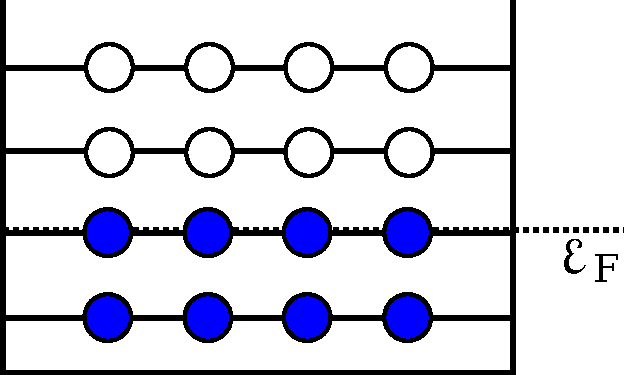
\includegraphics[height=4cm]{manybody/IPM.pdf}}}$
  \caption{A depiction of the closed-shell reference state in the independent particle model.  Each horizontal line represents a shell of single-particle orbits, represented by circles, and the dotted line represents the Fermi level which separates the unoccupied \textit{particle} states from the occupied \textit{hole} states.}
  \label{fig:reference_state}
\end{figure}

Any other Slater determinant can be constructed relative to this reference state by adding particles and/or removing holes.  A Slater determinant with $A$ particles added and $B$ holes removed from reference state is known as a $\ph{A}{B}$ excitation.  A $\ph{1}{1}$ state is constructed by removing a particle in the occupied state $i$ and adding a particle in the unoccupied state $a$,
\begin{equation} \label{eq:1p1h_ket_states}
  \ket{\Phi^{a}_{i}} &\equiv \co{a}\ao{i}\ket{\Phi}.
\end{equation}
Equivalently, a $\ph{2}{2}$ state is constructed by removing particles in states $i$ and $j$ then adding them to states $b$ and $a$,
\begin{equation} \label{eq:2p2h_ket_states}
  \ket{\Phi^{ab}_{ij}} &\equiv \co{a}\co{b}\ao{j}\ao{i}\ket{\Phi}.
\end{equation}
The number of creation and annihilation operators doesn't neccessarily have to be equal.  For instance, a single particle can be added on top of the reference state with a single creation operator,
\begin{equation} \label{eq:1p_ket_states}
  \ket{\Phi^{a}} &\equiv \co{a}\ket{\Phi},
\end{equation}
and a particle can be removed with a single annihilation operator,
\begin{equation} \label{eq:1h_ket_states}
  \ket{\Phi_{i}} &\equiv \ao{i}\ket{\Phi}.
\end{equation}

\begin{figure}
  \centering
  \begin{subfigure}{\textwidth}
    \centering
    $\ket{\Phi^{a}_{i}}\ = \vcenter{\hbox{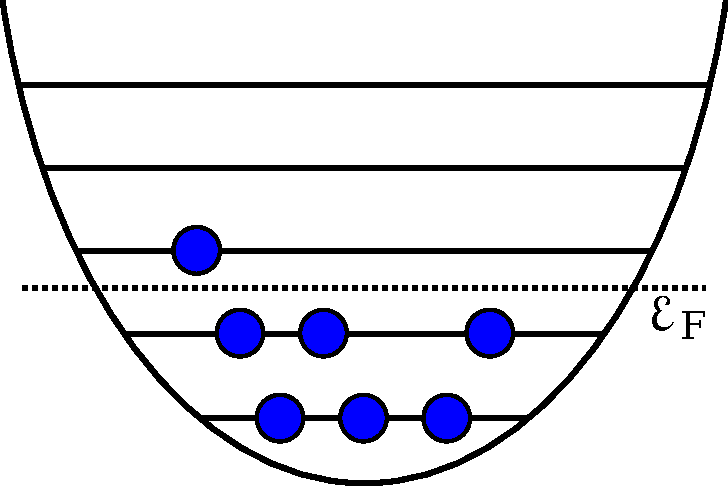
\includegraphics[height=3cm]{manybody/1p1h.pdf}}} \hspace{2cm} \ket{\Phi^{ab}_{ij}}\ = \vcenter{\hbox{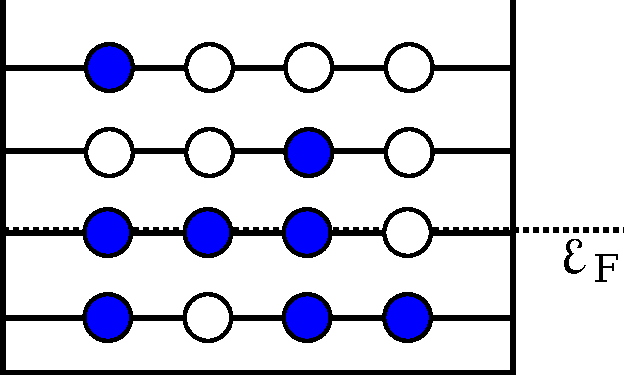
\includegraphics[height=3cm]{manybody/2p2h.pdf}}}$
  \end{subfigure}
  \vspace{0.5cm}
  
  \begin{subfigure}{\textwidth}
    \centering
    $\ket{\Phi^{a}}\ = \vcenter{\hbox{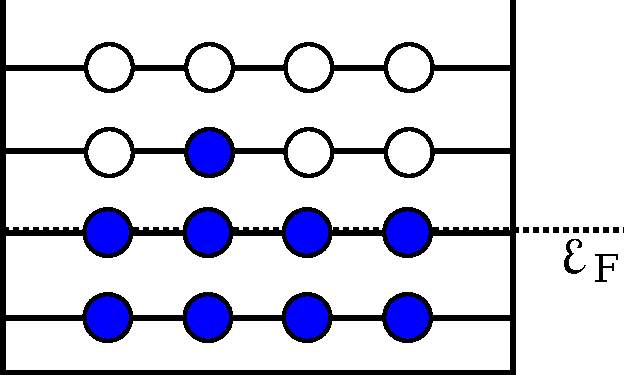
\includegraphics[height=3cm]{manybody/PA.pdf}}} \hspace{2cm} \ket{\Phi_{i}}\ = \vcenter{\hbox{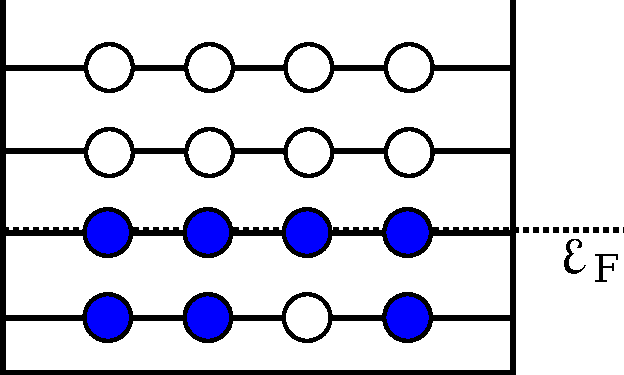
\includegraphics[height=3cm]{manybody/PR.pdf}}}$
  \end{subfigure}
  \caption{A depiction of $\ph{1}{1}$, $\ph{2}{2}$, $\ph{1}{0}$, and $\ph{0}{1}$ Slater determinants defined relative to the reference state in the independent particle model.}
  \label{fig:excitations}
\end{figure}
  
Using these definitions, hole-creation and particle-annihilation operators vanish when acting on the Fermi vacuum from the left, $\co{i}\refket=\ao{a}\refket=0$. Conversely, hole-annihilation and particle-creation operators vanish when acting on the Fermi vacuum from the right, $\refbra\ao{i}=\refbra\co{a}=0$.

These results can be exploited to simplify expressions involving strings of creation and annihilation operators by a procedure called \textit{normal ordering} with respect to the Fermi vacuum. Denoted by $\normord{\cdots}$, normal ordering permutes a string of creation and annihilation operators so that hole-annihilation and particle-creation operators are to the left of hole-creation and particle-annihilation operators, which guarantees that normal ordered operators vanish on the Fermi vacuum, $\refbra\normord{\cdots} = 0$ and $\normord{\cdots}\refket = 0$.
\begin{equation} \label{eq:normorddef}
  \normord{\co{j}\cdots\ao{i}\cdots\ao{b}\cdots\co{a}} = (-1)^{\sigma}\ao{i}\cdots\co{a}\cdots\co{j}\cdots\ao{b},
\end{equation}
where $\sigma$ is the number of two-state permutations required to do the normal ordering.


\section{Wick's Theorem} \label{section:wicks_theorem}
At this point, the many-body problem has been reduced to computing long strings of creation and annihilation operators between the normal-ordered Hamiltonian and the correlated wave function using Eq.\ \eqref{eq:anticommutation}.  Instead of using a brute-force approach by permuting over and over, a further simplification known as \textit{Wick's theorem} \cite{WICK1950} can be introduced.  A Wick contraction of two operators with respect to the reference state is defined as
\begin{equation} \label{eq:wick1}
  \contraction[1.0ex]{}{\hat{A}}{}{\hat{B}}
  \hat{A}\hat{B} = \hat{A}\hat{B} - \normord{\hat{A}\hat{B}}.
\end{equation}
Which, given the definition in Eq.\ \eqref{eq:normorddef} and the anticommutation relations int Eq.\ \eqref{eq:anticommutation}, means that the only nonzero contractions are of the form,
\begin{equation} \label{eq:wick2}
  \contraction[1.0ex]{}{\hat{a}}{^{\dagger}_{i}}{\hat{a}}
  \hat{a}^{\dagger}_{i}\hat{a}_{j} = \delta_{ij} \hspace{1.0cm} \text{and} \hspace{1.0cm}
  \contraction[1.0ex]{}{\hat{a}}{_{a}}{\hat{a}}
  \hat{a}_{a}\hat{a}_{b}^{\dagger} = \delta_{ab}.
\end{equation}
Because contracted operators simply represent a Kronecker delta, they can be removed from a normal ordered product by permuting the product $\sigma$ times so that the contracted operators are next to each other,
\begin{equation} \label{eq:wick3}
  \contraction[1.0ex]{\{ \hat{A}\cdots}{\hat{B}}{\cdots}{\hat{C}}
  \{ \hat{A}\cdots\hat{B}\cdots\hat{C}\cdots\hat{D} \} = (-1)^{\sigma}
  \contraction[1.0ex]{\{ \hat{A}\cdots}{\hat{B}}{}{\hat{C}}
  \{ \hat{A}\cdots\hat{B}\hat{C}\cdots\hat{D} \} = (-1)^{\sigma}
  \contraction[1.0ex]{}{\hat{B}}{}{\hat{C}}
  \hat{B}\hat{C}\{ \hat{A}\cdots\hat{D} \}.
\end{equation}
These different definitions for operator manipulation come together to define the time-independent Wick's theorem, which reformulates a product of operators as the sum of its normal-ordered form and all possible contractions of its normal-ordered form,
\begin{equation} \label{eq:wick4}
  \hat{A}\hat{B}\hat{C}\cdots\ =\ \normord{\hat{A}\hat{B}\hat{C}\cdots}\
  +\ \sum_{\mathclap{\substack{\text{one-} \\ \text{contractions}}}}
  \contraction[1.0ex]{\{ }{\hat{A}}{\hat{B}\hat{C}}{\cdots}
  \{ \hat{A}\hat{B}\hat{C}\cdots \}\
  +\ \sum_{\mathclap{\substack{\text{two-} \\ \text{contractions}}}}
  \contraction[0.8ex]{\{ }{\hat{A}}{\hat{B}\hat{C}}{\cdots}
  \contraction[1.2ex]{\{ \hat{A}}{\hat{B}}{\hat{C}\cdots}{}
  \{ \hat{A}\hat{B}\hat{C}\cdots \}\
  +\ \cdots\ +\ \sum_{\mathclap{\substack{\text{all-} \\ \text{contractions}}}}
  \contraction[0.6ex]{\{ }{\hat{A}}{\hat{B}\hat{C}}{\cdots}
  \contraction[1.0ex]{\{ \hat{A}}{\hat{B}}{\hat{C}\cdots}{\ }
  \contraction[1.4ex]{\{ \hat{A}\hat{B}}{\hat{C}}{\cdots\ \ \ }{}
  \{ \hat{A}\hat{B}\hat{C}\cdots\ \ \ \}.
\end{equation}

Wick's theorem is incredibly useful in many-body techniques because complicated expressions of operators can be expressed as diagrams that are easy to compute with simple diagrammatic rules which correspond to Eqs.\ \eqref{eq:anticommutation},\eqref{eq:wick2}, and \eqref{eq:wick3}.  These diagrammatic techniques are an integral component to deriving expressions used in this work, and their underlying rules are extensively discussed in \cite{SHAVITT2009}.

A powerful application of Wick's theorem is to rewrite the Hamiltonian in Eq.\ \eqref{eq:hamiltonian} as a sum of normal-ordered operators in the form of Eq.\ \eqref{eq:wick4},
\begin{equation} \label{eq:HamN}
  \Ham = E_{0} + \sum_{\mathclap{pq}}\fint{p}{q}\normord{\co{p}\ao{q}} + \frac{1}{4}\sum_{\mathclap{pqrs}}\vint{pq}{rs}\normord{\co{p}\co{q}\ao{s}\ao{r}} + \frac{1}{36}\sum_{\mathclap{pqrstu}}\wint{pqr}{stu}\normord{\co{p}\co{q}\co{r}\ao{u}\ao{t}\ao{s}} + \cdots.
\end{equation}
This form of the Hamiltonian can be split into a zero-body component $E_{0}$, known as the \textit{reference energy}, and the remaining \textit{normal-ordered Hamiltonian}, $\HamN$,
\begin{equation} \label{eq:HamN1}
  \HamN = \sum_{\mathclap{pq}}\fint{p}{q}\normord{\co{p}\ao{q}} + \frac{1}{4}\sum_{\mathclap{pqrs}}\vint{pq}{rs}\normord{\co{p}\co{q}\ao{s}\ao{r}} + \frac{1}{36}\sum_{\mathclap{pqrstu}}\wint{pqr}{stu}\normord{\co{p}\co{q}\co{r}\ao{u}\ao{t}\ao{s}} + \cdots.
\end{equation}

The reference energy, $E_{0}$, contains fully-contracted terms, and because the Hamiltonian operators are ordered so that the creation operators appear before the annihilations operators, only terms that contract \textit{hole} states in the form $\contraction[0.8ex]{\{ \cdots}{\hat{a}}{^{\dagger}_{i}\cdots}{\hat{a}}\{ \cdots\co{i}\cdots\ao{j}\cdots \}$ are nonzero.  Therefore, the zero-body component of the normal ordered Hamiltonian can be written as a sums over all hole states for each component of the original Hamiltonian,
\begin{equation} \label{eq:HamN_0}
  E_{0} = \sum_{\mathclap{i}}\Hint{1}{i}{i} + \frac{1}{2}\sum_{\mathclap{ij}}\Hint{2}{ij}{ij} + \frac{1}{6}\sum_{\mathclap{ijk}}\Hint{3}{ijk}{ijk} \cdots.
\end{equation}
In a compact diagrammatic form, this sum can be drawn as the sum of connected vertices (\raisebox{-5pt}{\mbox{
\includegraphics[height=15pt]{diagrams/Hamiltonian/Hamiltonian-figure12.pdf}}}, \raisebox{-5pt}{\mbox{
\includegraphics[height=15pt]{diagrams/Hamiltonian/Hamiltonian-figure13.pdf}}}, etc...) corresponding to the components of the original Hamiltonian in Eq.\ \eqref{eq:hamiltonian},
\begin{equation}
  E_{0} = \diagram{Hamiltonian/Hamiltonian-figure0} + \diagram{Hamiltonian/Hamiltonian-figure1} + \diagram{Hamiltonian/Hamiltonian-figure2} + \cdots.
\end{equation}
The number of lines connected to each vertex defines its type such that the single vertex corresponds to the one-body Hamiltonian, the double vertex corresponds to the two-body Hamiltonian, etc...  The looped lines represent a sum over all hole states.  The reference energy is also equivalent to the Hamiltonian expectation value for the reference state,
\begin{equation} \label{eq:E_ref}
  E_{0} = \element{\Ref}{\Ham}{\Ref}.
\end{equation}

The second component of the normal-ordered Hamiltonian, $\fint{p}{q}\normord{\co{p}\ao{q}}$, contains terms that have all operators contracted except for one pair.  Like the fully-contracted term, these contractions must involve only hole states,
\begin{equation} \label{eq:HamN_1}
  \fint{p}{q} = \Hint{1}{p}{q} + \sum_{\mathclap{i}}\Hint{2}{pi}{qi} + \frac{1}{2}\sum_{\mathclap{ij}}\Hint{3}{pij}{qij} + \cdots.
\end{equation}
In diagrammatic notation, the uncontracted pair of operators is represented as two external lines connected to each vertex which, because they are generic states, are drawn as unoriented lines,
\begin{equation}
  \diagram{Hamiltonian/Hamiltonian-figure3} = \diagram{Hamiltonian/Hamiltonian-figure4} + \diagram{Hamiltonian/Hamiltonian-figure5} + \diagram{Hamiltonian/Hamiltonian-figure6} + \cdots.
\end{equation}
When a line represents a particle state, it will contain an arrow directed upwards while a line representing a hole state will contain an arrow directed downwards.

The two-body term, $\vint{pq}{rs}\normord{\co{p}\co{q}\ao{s}\ao{r}}$, follows in the same manner such that it represents all terms of the original Hamiltonian with all but two pairs of operators contracted.  Like the zero-body and one-body terms, the two-body term contains the original two-body term $\HamB{2}$ as well as density-dependent terms that sum over hole states in higher-body Hamiltonian terms, leaving four external lines for each diagram vertex,
\begin{align} \label{eq:HamN_2}
  \vint{pq}{rs} &= \Hint{2}{pq}{rs} + \sum_{\mathclap{i}}\Hint{3}{pqi}{rsi} + \cdots \notag \\
  \diagram{Hamiltonian/Hamiltonian-figure7} &= \diagram{Hamiltonian/Hamiltonian-figure8} + \diagram{Hamiltonian/Hamiltonian-figure9} + \cdots.
\end{align}

Three- and four-body normal-ordered terms can also be calculated by following the same procedure, but in practice are truncated at the two- or three-body level.  Because normal ordering the Hamiltonian has the effect of shuffling higher-order interactions into lower-order terms, it becomes feasible to include computationally expensive many-body interactions as normal-ordered few-body interactions.  Also, it reorganizes many-body correlations into the reference state so that additional correlations around the Fermi surface can be treated as a perturbation.  Therefore, from this point forward, the many-body problem will be formulated in terms of the normal-ordered terms in Eq.\ \eqref{eq:HamN}, and the bare interactions will be truncated beyond the three-body level for computational feasibility.  Electronic systems are naturally truncated at the level of the two-body Coulomb interaction, while nuclear systems can be successfully described with the two-body normal-ordered piece of the three-body force, in the form of Eq.\ \eqref{eq:HamN_2}.

With this new partition, the many-body Schr\"{o}dinger equation for the ground state $\ket{\Corr}$ can be written in terms of the normal-ordered Hamiltonian as,
\begin{gather} \label{eq:normal_schrodinger}
  \Ham\ket{\Psi} = (E_{0} + \HamN)\ket{\Psi} = E\ket{\Psi} \notag \\
  \longrightarrow\ \ \HamN\ket{\Psi} = (E - E_{0})\ket{\Psi} = \Ecorr\ket{\Psi},
\end{gather}
where $\Ecorr$ is known as the \textit{correlation energy}.

Now that the many-body quantum problem has been formulated, different approaches to solving that problem can be proposed and analyzed.  Because taking account of correlations from all particles simultaneously is a demanding--and for some systems, computationally impossible--endeavor, methods for solving the many-body Schr\"{o}dinger equation should be systematically improvable. Successful methods with this quality incorporate the most dominant correlations in lower-order solutions and approach the exact solution when more and more orders are included.

\section{Hartree--Fock Method} \label{section:hartree-fock}
A successful, first-order approximation to any many-body method comes from noticing that each individual particle feels a mean-field potential from the cumulative interactions with all the other particles.  The \textit{Hartree-Fock} (HF) method \cite{HARTREE1928,FOCK1930} aims to transform the original single-particle basis to a Hartree-Fock basis where each orbital is the eigenfunction of its corresponding mean-field.  Because the transformation of a single orbital changes its effect on every other particle, this process must be performed iteratively until self-consistency between all the orbitals is reached, which is why this method is also known as the \textit{Self-Consistent Field} (SCF) method.

This mean-field picture results from the following procedure.  It begins by minimizing the reference energy with respect to the reference state.  This functional is just the zero-body piece of the normal-ordered Hamiltonian,
\begin{equation}
  E_{\text{HF}}\left[ \Ref \right] = \element{\Ref}{\Ham}{\Ref} = \sum_{\mathclap{i}}\Hint{1}{i}{i} + \frac{1}{2}\sum_{\mathclap{ij}}\Hint{2}{ij}{ij} + \frac{1}{6}\sum_{\mathclap{ijk}}\Hint{3}{ijk}{ijk}.
\end{equation}
Transforming the reference determinant can be accomplished by rotating the state within the single-particle basis by use of the \textit{Thouless theorem} \cite{THOULESS1960225}, which states that any Slater determinant can be written as the product of any other Slater determinant and an exponentiated single-excitation operator,
\begin{equation} \label{eq:thouless}
  \ket{\Phi'} = e^{\hat{C}_{1}}\refket, \hspace{1cm} \text{where\ \ } \hat{C}_{1} = \sum_{a i}C^{a}_{i}\normord{ \co{a}\ao{i} }.
\end{equation}
If the difference between the two Slater determinants is dominated by single excitations, this transformation can be approximated by expanding the exponential and ignoring higher-order terms,
\begin{equation} \label{eq:thouless_limit}
  \ket{\Phi'} \simeq \left( 1 + \sum_{a i}C^{a}_{i}\normord{ \co{a}\ao{i} } \right)\refket.
\end{equation}

The reference energy functional can now be written as a sum of the original reference state and new terms that incorporate the single-excitation variation,
\begin{equation} \label{eq:hf_thouless}
  E_{\text{HF}}\left[ \Phi' \right] = \element{\Phi'}{\Ham}{\Phi'} \simeq E_{\text{HF}}\left[ \Ref \right] + \sum_{a i}C^{a}_{i}\refbra\Ham\ket{\Phi^{a}_{i}} + \sum_{a i}C^{a*}_{\ i}\bra{\Phi^{a}_{i}}\Ham\refket.
\end{equation}
The minimum of this functional is found by differentiating the expression with respect to the coefficients $C^{a}_{i}$ and setting the result to zero,
\begin{equation} \label{eq:del_hf_thouless}
  \delta E_{\text{HF}}\left[ \Phi' \right] \simeq \sum_{a i}\delta C^{a}_{i}\refbra\Ham\ket{\Phi^{a}_{i}} + \sum_{a i}\delta C^{a*}_{\ i}\bra{\Phi^{a}_{i}}\Ham\refket = 0.
\end{equation}

Because this expression is Hermitian, both terms must vanish independently so that,
\begin{equation} \label{eq:brillouin}
  \refbra\Ham\ket{\Phi^{a}_{i}} = \bra{\Phi^{a}_{i}}\Ham\refket = 0.
\end{equation}
This condition is the result of the \textit{Brillouin theorem} \cite{BRILLOUIN1932}, which states that the Hamiltonian matrix element must vanish between an optimized Hartree-Fock ground state and any single excitation from it. The Brillouin condition is satisfied by diagonalizing the one-body piece of the normal-ordered Hamiltonian $\fint{p}{q}$ (Eq.\ \eqref{eq:HamN_1}), known as the \textit{Fock} operator, such that off-diagonal pieces like $\refbra\Ham\ket{\Phi^{a}_{i}} = \fint{i}{a}$ and $\bra{\Phi^{a}_{i}}\Ham\refket = \fint{a}{i}$ vanish.  Diagonalizing the Fock operator can be written schematically as,
\begin{gather} \label{eq:fock_operator}
  \varepsilon^{p}_{q}\delta_{pq}\ \ \longleftarrow\ \ \Hint{1}{p}{q} + \sum_{\mathclap{i}}\Hint{2}{pi}{qi} + \frac{1}{2}\sum_{\mathclap{ij}}\Hint{3}{pij}{qij} \notag \\
  \diagram{Hamiltonian/Hamiltonian-figure3}\ \ \longleftarrow\ \ \diagram{Hamiltonian/Hamiltonian-figure4} + \diagram{Hamiltonian/Hamiltonian-figure5} + \diagram{Hamiltonian/Hamiltonian-figure6},
\end{gather}
where $\varepsilon^{p}_{q}$ is the eigenvalue of the Fock operator, and its diagrammatic form vanishes when the external indices differ.

A practical way of solving this system of equations is to express each new orbital in the unknown Hatree-Fock basis, $\ket{p'} \equiv \phi_{p'}\left(\mathbf{r}\right)$, denoted with primed labels, as a linear combination of the known single-particle basis states, $\ket{p} \equiv \phi_{p}\left(\mathbf{r}\right)$, denoted without primed labels.  These two bases are related by a unitary transformation $C^{p}_{p'} \equiv \braket{p}{p'}$,
\begin{equation} \label{eq:fock_matrix_prime}
  \ket{p'} = \sum_{p}\braket{p}{p'}\ket{p} = \sum_{p}C^{p}_{p'}\ket{p}.
\end{equation}
Then the Fock matrix can be written in terms of the Hartree-Fock basis,
\begin{gather}
  \fint{p'}{q'} = \Hint{1}{p'}{q'} + \sum_{\mathclap{i'}}\Hint{2}{p'i'}{q'i'} + \frac{1}{2}\sum_{\mathclap{i'j'}}\Hint{3}{p'i'j'}{q'i'j'} \notag \\
  = \sum_{\mathclap{pq}}C^{p'*}_{p}\Hint{1}{p}{q}C^{q}_{q'} + \sum_{\mathclap{\substack{i' \\ prqs}}}C^{p'*}_{p}C^{i'*}_{r}\Hint{2}{pr}{qs}C^{q}_{q'}C^{s}_{i'} + \frac{1}{2}\sum_{\mathclap{\substack{i'j' \\ prsqtu}}}C^{p'*}_{p}C^{i'*}_{r}C^{j'*}_{s}\Hint{3}{prs}{qtu}C^{q}_{q'}C^{t}_{i'}C^{u}_{j'}.
\end{gather}
Defining the first-order density matrix $\gamma^{p}_{q}$ as the product of expansion coefficients, summed over all shared hole states,
\begin{equation}
  \gamma^{p}_{q} = \sum_{i'}C^{p}_{i'}C^{i'*}_{q},
\end{equation}
Eq.\ \eqref{eq:fock_matrix_prime} is simplified to,
\begin{equation}
  \fint{p'}{q'} = \sum_{\mathclap{pq}}C^{p'*}_{p}\left[ \Hint{1}{p}{q} + \sum_{\mathclap{rs}}\gamma^{r}_{s}\Hint{2}{pr}{qs} + \frac{1}{2}\sum_{\mathclap{rstu}}\gamma^{r}_{t}\gamma^{s}_{u}\Hint{3}{prs}{qtu} \right]C^{q}_{q'}\ \ \longrightarrow\ \ \varepsilon^{p'}_{q'}\delta_{p'q'}.
\end{equation}
Therefore, the Hartree-Fock equations are ultimately expressed as an eigenvalue problem according to Eq.\ \eqref{eq:fock_operator} where the matrix to diagonalize is the Fock matrix in the form,
\begin{equation}
  \hat{F}^{p}_{q}\left(\hat{C}\right) = \Hint{1}{p}{q} + \sum_{\mathclap{rs}}\gamma^{s}_{r}\Hint{2}{pr}{qs} + \frac{1}{2}\sum_{\mathclap{rstu}}\gamma^{t}_{r}\gamma^{u}_{s}\Hint{3}{prs}{qtu},
\end{equation}
and the matrix of coefficients, $\hat{C} = C^{p}_{p'}$, is the unitary operator that transforms the matrix to a diagonal form,
\begin{equation}
  \sum_{\mathclap{pq}}C^{p'*}_{p}F^{p}_{q}\left(\hat{C}\right)C^{q}_{q'} = \varepsilon^{p'}_{q'}\delta_{p'q'}
\end{equation}
The iterative nature of the solution comes from the dependence of the Fock matrix on the transformation coefficients. These Hartree-Fock equations are solved numerically by using an iterative algorithm where the Fock matrix is built using a known set of coefficients and diagonalized to obtain an updated set of coefficients.  This process is repeated until the unitary set of coefficients is unchanged within a certain tolerance.  For most calculations, using the identity matrix as an initial guess for the coefficients is sufficient.  To improve the rate of convergence, techniques such as the direct inversion of the iterative subspace (DIIS) \cite{PULAY1980393,PULAY1982556} or Broyden's method \cite{BROYDEN1965557} can be implemented.  And, to avoid any oscillatory behavior around the solution, techniques such as the level-shifting method or \textit{ad hoc} linear mixing can be implemented to dampen the large changes between iterations.

To make use of the HF solution as the reference state for post-HF calculations, the Hamiltonian matrix elements must be transformed to the new basis and the normal-ordered pieces redefined to account for the additional reordering of one-particle correlations into the HF energy.  The one-body piece from Eq.\ \eqref{eq:HamN_1} is simply the resulting eigenvalues of the diagonalized Fock matrix,
\begin{equation} \label{eq:HF_Ham_1}
  \fint{p'}{q'} = \varepsilon^{p'}_{q'}\delta_{p'q'}.
\end{equation}
For the two-body term, Eq.\ \eqref{eq:HamN_2}, first the density-dependent component of the three-body interaction is written with the first-order density matrix.  Then the remaining states are transformed according to Eq.\ \eqref{eq:fock_matrix_prime},
\begin{equation} \label{eq:HF_Ham_2}
  \vint{p'q'}{r's'} = \sum_{\mathclap{pqrs}} C^{p'*}_{p}C^{q'*}_{q}\left(\Hint{2}{pq}{rs} + \Hint{3}{pqt}{rsu}\gamma^{u}_{t}\right)C^{r}_{r'}C^{s}_{s'}.
\end{equation}
The reference energy from Eqns.\ \eqref{eq:HamN_0} and \eqref{eq:E_ref} can be written in terms of the transformed one- and two-body Hamiltonian, Eqns.\ \eqref{eq:HamN_1} and \eqref{eq:HamN_2}, and the original three-body term using first-order density matrices,
\begin{equation} \label{eq:EF_Ham_0}
  E_{0} = \sum_{\mathclap{i'}}\varepsilon^{i'}_{i'} - \frac{1}{2}\sum_{\mathclap{i'j'}}\vint{i'j'}{i'j'} + \frac{1}{6}\ \sum_{\mathclap{pqrstu}}\Hint{3}{pqr}{stu}\gamma^{s}_{p}\gamma^{t}_{q}\gamma^{r}_{u}.
\end{equation}
Additionally, any operators that are constructed in the original basis must be transformed in a similar manner.  For example, a one-body operator $\hat{O}$ in the Hartree-Fock basis is,
\begin{gather}
  \hat{O} = \sum_{\mathclap{p'q'}}\opint{}{p'}{q'}\normord{\co{p'}\ao{q'}} = \sum_{\mathclap{p'q'pq}}C^{p'*}_{p}\opint{}{p}{q}C^{q}_{q'}\normord{\co{p'}\ao{q'}} \notag \\
  \longrightarrow\ \ \ \opint{}{p'}{q'} = \sum_{\mathclap{pq}}C^{p'*}_{p}\opint{}{p}{q}C^{q}_{q'}.
\end{gather}

Because the Hartree-Fock basis is diagonal in the one-body piece of the Hamiltonian, any terms that include off-diagonal elements automatically vanish, greatly simplifying any post-Hartree-Fock methods.  From this point on, all calculations will use the Hartree-Fock basis unless stated otherwise, and prime symbols will be omitted.


\section{Configuration-Interaction} \label{section:configuration_interaction}
The most generic way to write a correlated wave function in a given basis is as a linear combination of all possible Slater determinants.  This expansion can, in principle, consist of the $\ph{0}{0}$ reference state and all possible $\ph{N}{N}$ excitations up to $\ph{A}{A}$ excitations,
\begin{equation} \label{eq:ci_expansion}
  \ket{\Psi_{\nu}} = \sum_{\nu_{i}}^{\mathcal{N}}C_{\nu_{i}}\ket{\Phi_{\nu_{i}}} = C_{0}\ket{\Phi_{0}} + \sum_{N=1}^{A}\left(\frac{1}{N!}\right)^2 \sum_{\substack{a_{1} \ldots a_{N} \\ i_{1} \ldots i_{N}}} C^{a_{1} \ldots a_{N}}_{i_{1} \ldots i_{N}}\ket{\Phi^{a_{1} \ldots a_{N}}_{i_{1} \ldots i_{N}}}.
\end{equation}
Using this form of the wave function in Eq.\ \eqref{eq:ci_expansion}, the normal-ordered Schr\"{o}dinger equation can be reformulated as a standard matrix eigenvalue problem,
\begin{gather}
  \HamN\ket{\Psi_{\nu}} = \Ecorr_{\nu}\ket{\Psi_{\nu}}\ \ \longrightarrow\ \ \element{\Psi_{\mu}}{\HamN}{\Psi_{\nu}} = \Ecorr_{\nu}\braket{\Psi_{\mu}}{\Psi_{\nu}} \notag \\
  = \sum_{\mathclap{\mu_{i}\nu_{i}}}C^{*}_{\mu_{i}}\element{\Phi_{\mu_{i}}}{\HamN}{\Phi_{\nu_{i}}}C_{\nu_{i}} = \Ecorr_{\nu}\sum_{\mathclap{\mu_{i}\nu_{i}}}C^{*}_{\mu_{i}}C_{\nu_{i}}\delta_{\mu_{i}\nu_{i}} \notag \\
  \longrightarrow\ \ \mathbf{C}^{\text{T}}_{\mu}\left(\element{\Phi_{\mu_{i}}}{\HamN}{\Phi_{\nu_{i}}} - \Ecorr_{\nu}\mathbf{I}\right)\mathbf{C}_{\nu} = 0.
\end{gather}
In this case, the matrix elements are Hamiltonian terms that connect two Slater determinants, and the eigenvectors are the ground and excited states in the form of Eq.\ \eqref{eq:ci_expansion}.  The matrix elements can be found with the help of the Slater-Condon rules \cite{SLATER1929,CONDON1930} which, because the Hamiltonian is restricted to one- and two-body terms, require that any terms connecting Slater determinants which differ by more than two single-particle states vanish.  Also, because the one-body Hamiltonian is diagonal in the Hartree-Fock basis, it only contributes to diagonal elements of the CI matrix.  Some examples of these matrix elements are,
\begin{gather} \label{eq:slater_condon}
  \element{\Phi^{a}_{i}}{\Ham}{\Phi^{a}_{i}} = \Edenom{}{a} - \Edenom{}{i} - \vint{ia}{ia}, \notag \\
  \element{\Phi^{ab}_{ij}}{\Ham}{\Phi^{cd}_{ij}} = \vint{ab}{cd}, \notag \\
  \element{\Phi^{abc}_{ijk}}{\Ham}{\Phi^{abd}_{ijl}} = -\vint{lc}{kd}.
\end{gather}

Because the configuration-interaction method exhaustively captures all the correlations of a many-body system, it is considered an ``exact'' method within a certain model space and becomes truly exact as the number of single-particle states is increased to infinity.  However, there is a price to pay for this exactness.  The number of Slater determinants in a certain model space, $\mathcal{N}$, scales factorially according to Eq.\ \eqref{eq:factorialscaling} and the configuration-interaction matrix scales as $\mathcal{N}^{2}$.  For sufficiently-sized model spaces, the memory required for this matrix quickly becomes unmanagable even for the largest supercomputers, see Fig.\ \ref{fig:fciscaling}.
\begin{figure}[h]
  \centering
  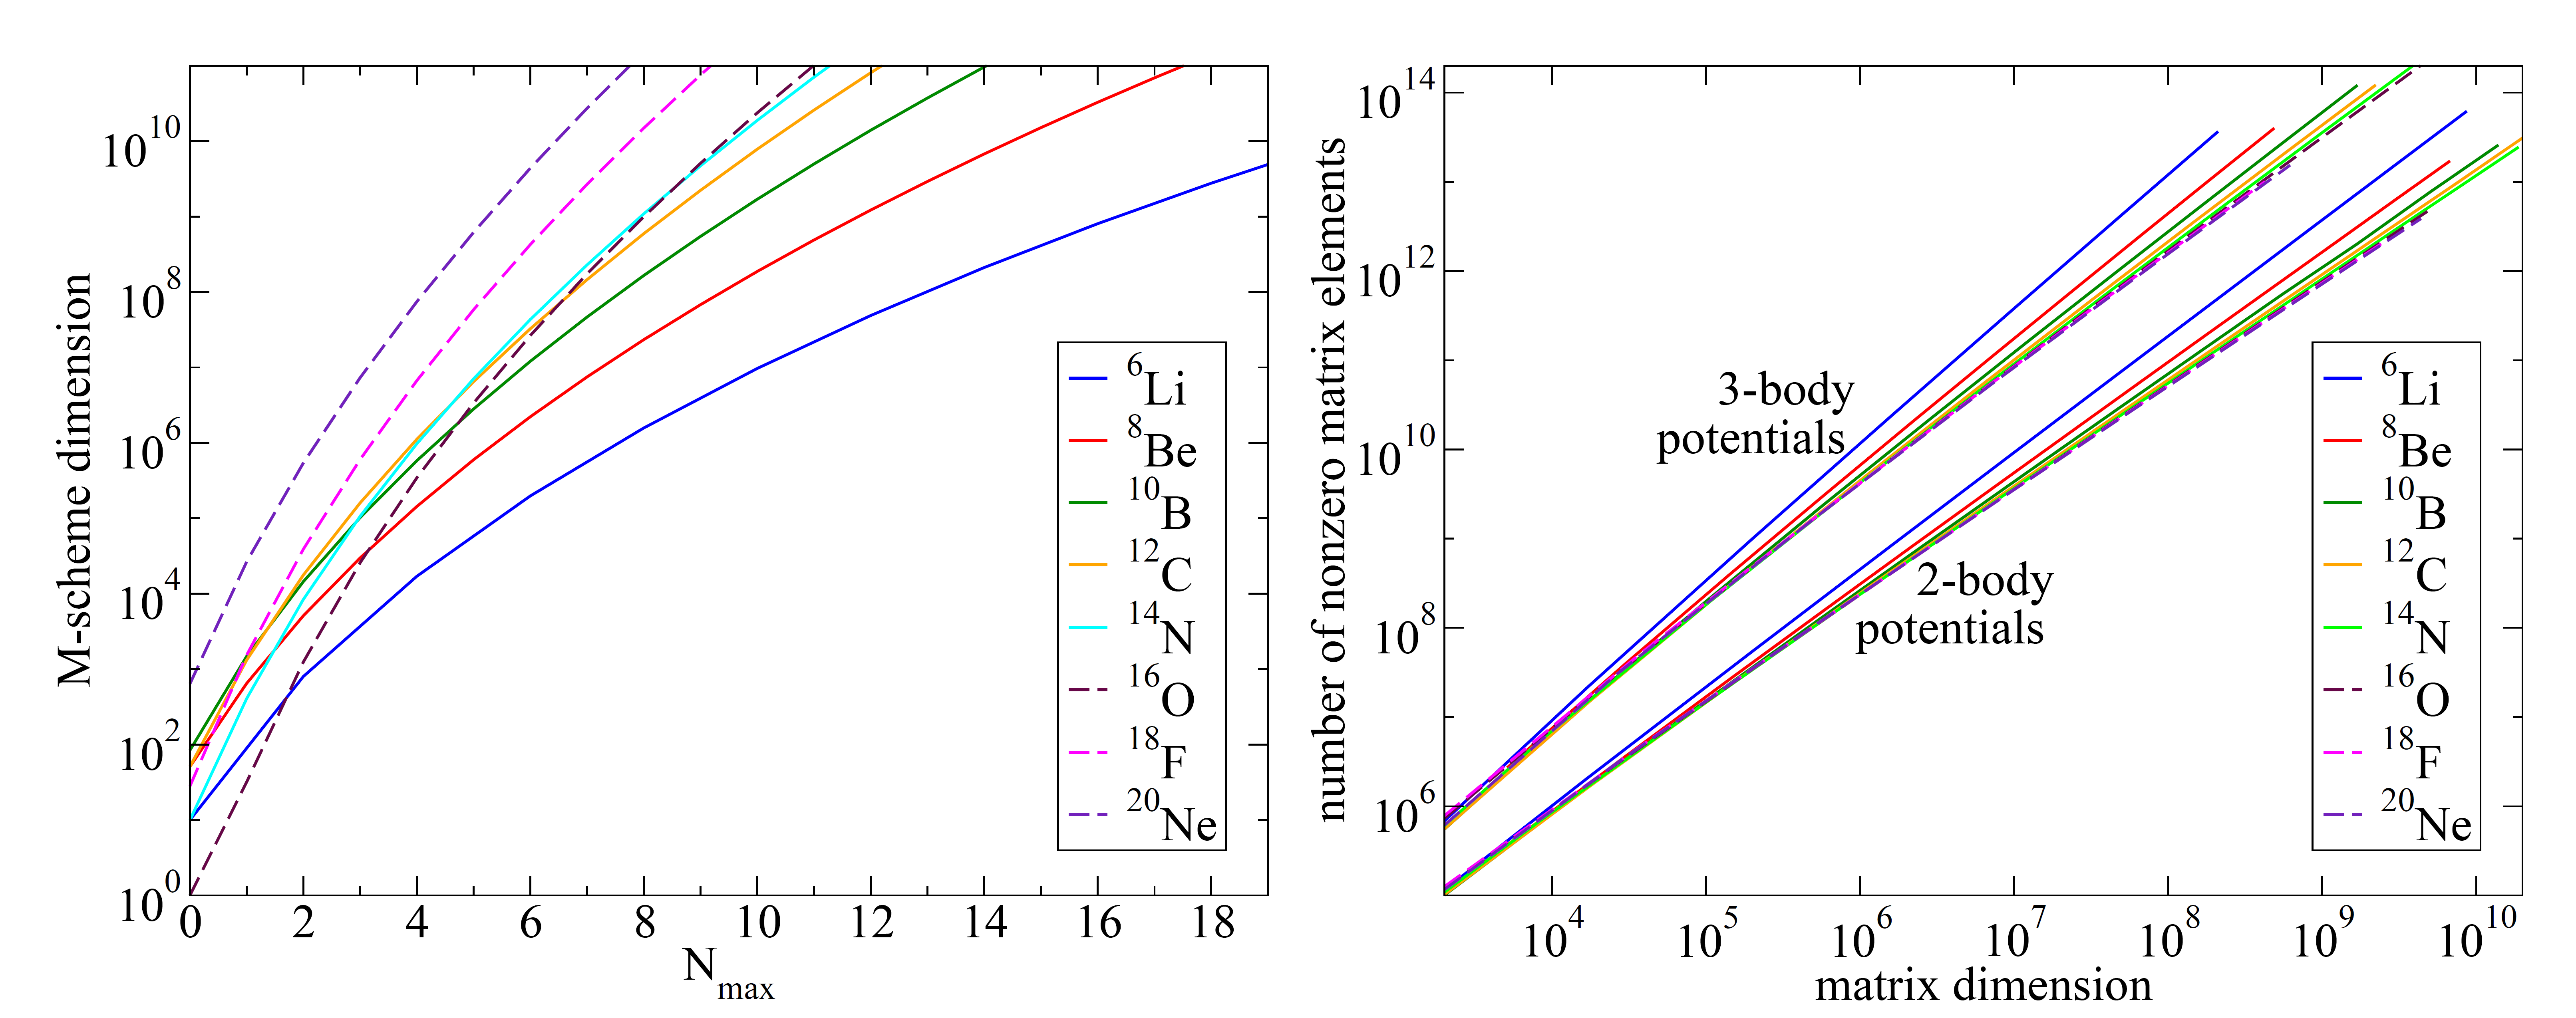
\includegraphics[width=\textwidth]{manybody/FCIscaling.png}
  \caption{Scaling of the matrix size and number of non-zero matrix elements for nuclear CI calculations of light nuclei.  Even for modestly-sized model spaces, the memory requirements approach the limit of petascale supercomputers ($\sim 10^{10}$).  Figure taken from \cite{SHAO2016}.}
  \label{fig:fciscaling}
\end{figure}

However, for a reference state that is a good approximation to the true ground state, few-body excitations generally dominate the wave functions for low-lying states \cite{SHERRILL1999143}.  This can be exploited by truncating the expansion in Eq.\ \eqref{eq:ci_expansion}.  Owing to the two-body nature of the interaction, the lowest appropriate truncation is also at the two-body level, known as configuration interaction with singles and doubles (CISD),
\begin{equation} \label{eq:cisd_expansion}
  \ket{\Psi_{\nu}} = C_{0}\ket{\Phi_{0}} + \sum_{\mathclap{a i}} C^{a}_{i}\ket{\Phi^{a}_{i}} + \frac{1}{4}\sum_{\mathclap{a b i j}} C^{ab}_{ij}\ket{\Phi^{ab}_{ij}}.
\end{equation}
This is a very straightforward and tractable way to approximate the many-body Schr\"{o}dinger equation, and it can be systematically improved by adding more excitations such as triples (CISDT) or triples and quadruples (CISDTQ).  But the drawback to this simplicity is that any truncated CI method is not size-extensive such that any extensive property of a system, like the energy, would scale with the size of the system.  A desirable many-body method will be both systematically improvable and size-extensive while maintaining computational feasibility.


\section{Many-Body Perturbation Theory} \label{section:MBPT}
One many-body method that is both size-extensive and systematically improvable treats particle-particle interactions as a perturbation to the mean-field potential and is known as many-body perturbation theory (MBPT) \cite{MOLLER1934,HUBBARD1957539,HUGENHOLTZ1957481,SHAVITT2009}.  The Hamiltonian is partitioned into a diagonal piece and the interaction piece,
\begin{gather} \label{eq:mbpt_hamiltonian}
  \Ham = \Ham_{0} + \hat{V},\ \ \text{with} \notag \\
  \Ham_{0} = E_{0} + \sum_{\mathclap{p}}\fint{p}{p}\normord{\co{p}\ao{p}}\ \ \text{and} \notag \\
  \hat{V} = \frac{1}{4}\sum_{\mathclap{pqrs}}\vint{pq}{rs}\normord{\co{p}\co{q}\ao{s}\ao{r}}.
\end{gather}
When not in the Hartree-Fock basis, the interaction piece has the additional off-diagonal Fock term, $\sum_{p\neq q}\fint{p}{q}\normord{\co{p}\ao{q}}$.  This means that the reference state is an eigenstate of the zero-order piece of the Hamiltonian,
\begin{equation}
  \Ham_{0}\refket = \left(E_{0} + \sum_{\mathclap{i}}\fint{i}{i}\normord{\co{i}\ao{i}}\right)\refket = \left(E_{0} + \sum_{\mathclap{i}}\Edenom{}{i}\right)\refket = E^{(0)}_{0}\refket.
\end{equation}
Using \textit{intermediate normalization}, which sets $\braket{\Ref}{\Psi} = 1$, the Schr\"{o}dinger equation, Eq.\ \eqref{eq:schrodinger} for the ground state becomes,
\begin{align}
  \refbra\mathop{(\Ham_{0} + \hat{V})}\corrket &= \refbra\Ham_{0}\corrket + \refbra\hat{V}\corrket = E\braket{\Phi}{\Psi} \notag \\
  &= E^{(0)}\braket{\Phi}{\Psi} + \refbra\hat{V}\corrket = E^{(0)} + \Delta E_{0} = E, \label{eq:mbpt_schrodinger}
\end{align}
where the energy difference is $\Delta E_{0} \equiv \refbra\hat{V}\corrket$.

Next, the projection operators $\hat{P}$ and $\hat{Q}$ can be introduced,
\begin{gather}
  \hat{P} = \ket{\Phi_{0}}\bra{\Phi_{0}}, \\
  \hat{Q} = \sum_{n\neq 0}\ket{\Phi_{n}}\bra{\Phi_{n}} = 1 - \ket{\Phi_{0}}\bra{\Phi_{0}}.
\end{gather}
The $\hat{P}$ operator isolates the reference-state component of any Slater determinant while the $\hat{Q}$ operator isolates all components \textit{except} the reference-state component out of any Slater determinant.  Both these operators are idempotent, which means that $\hat{P}^{2} = \hat{P}$ and $\hat{Q}^{2} = \hat{Q}$, and because of intermediate normalization, the correlated wave function can be written as $\ket{\Psi} = \mathop{(\hat{P} + \hat{Q})}\ket{\Psi} = \ket{\Phi} + \hat{Q}\ket{\Psi}$.  Also, both operators commute with the unperturbed part of the Hamiltonian, $\Ham_{0}\hat{P} = \hat{P}\Ham_{0}$ and $\Ham_{0}\hat{Q} = \hat{Q}\Ham_{0}$.  These identities can be applied to an alternate version of the Schr\"{o}dinger equation which defines a particular version of perturbation theory known as Raleigh-Schr\"{o}dinger perturbation theory (RSPT) \cite{RAYLEIGH1894,SCHRODINGER1926}. In this version, the zeroth-order energy $E^{(0)}$ is added to both sides of the Schr\"{o}dinger equation.  Acting with $\hat{Q}$ and rearranging terms gives,
\begin{gather}
  \hat{Q}\mathop{(E^{(0)} - \Ham_{0})}\ket{\Psi} = \hat{Q}\mathop{(E^{(0)} + \hat{V} - E)}\ket{\Psi} \notag \\
  \hat{Q}\mathop{(E^{(0)} - \Ham_{0})}\hat{Q}\ket{\Psi} = \hat{Q}\mathop{(\hat{V} - \Delta E_{0})}\ket{\Psi},
\end{gather}
where $\Delta E_{0} \equiv E - E^{(0)} = \refbra\hat{V}\corrket$.  The operator $\hat{Q}\mathop{(E^{(0)} - \Ham_{0})}\hat{Q}$ is invertible because $\mathop{(E^{(0)} - \Ham_{0})^{-1}}$ is never singular in $Q$-space.  Therefore, the operator $\hat{R}_{0} = \hat{Q}\mathop{(E^{(0)} - \Ham_{0})^{-1}}\hat{Q}$, known as the \textit{resolvent}, can be applied to both sides which gives,
\begin{equation}
  \hat{Q}\ket{\Psi} = \hat{R}_{0}\mathop{(\hat{V} - \Delta E_{0})}\ket{\Psi}.
\end{equation}
The left-hand side of this equation can be rewritten as $\hat{Q}\ket{\Psi} = \corrket - \refket$ to result in the generating equation for RSPT,
\begin{equation} \label{eq:MBPT_Q}
  \ket{\Psi} = \ket{\Phi} + \hat{R}_{0}\mathop{(\hat{V} - \Delta E_{0})}\ket{\Psi}.
\end{equation}
Because the single-particle states are eigenfunctions of the zeroth-order Hamiltonian, they are also eigenfunctions of the resolvent, with the resulting eigenvalues, $\Edenom{}{}$, are known as \textit{energy denominators}.  Applying the resolvent operator to any state orthogonal to the reference state, see Eqs.\ \eqref{eq:1p1h_ket_states} - \eqref{eq:1h_ket_states}, gives the following relation,
\begin{gather} \label{eq:energy_denominators}
  \hat{R}_{0}\stateket{a_{1}\cdots a_{N}}{i_{1}\cdots i_{N}} = \frac{1}{\Edenom{a_{1}\cdots a_{N}}{i_{1}\cdots i_{N}}}\stateket{a_{1}\cdots a_{N}}{i_{1}\cdots i_{N}},\ \ \text{where} \notag \\
  \Edenom{a_{1}\cdots a_{N}}{i_{1}\cdots i_{N}} = \varepsilon_{i_{1}} + \cdots + \varepsilon_{i_{N}} - \varepsilon_{a_{1}} - \cdots - \varepsilon_{a_{N}}.
\end{gather}

Equation \eqref{eq:MBPT_Q} can be iterated infinitely to give the solution for the fully correlated wave function,
\begin{equation} \label{eq:MBPT_wave1}
  \ket{\Psi} = \sum_{n=0}^{\infty}\left[\hat{R}_{0}\mathop{(\hat{V} - \Delta E_{0})}\right]^{n}\refket.
\end{equation}
Applying this form of the correlated wave function into Eq.\ \eqref{eq:mbpt_schrodinger} results in the energy difference,
\begin{equation} \label{eq:MBPT_energy1}
  \Delta E_{0} = \refbra\hat{V}\corrket = \sum_{n=0}^{\infty}\refbra\hat{V}\left[\hat{R}_{0}\mathop{(\hat{V} - \Delta E_{0})}\right]^{n}\refket
\end{equation}

The immediate problem with these equations is that the right-hand sides contain the target energy difference $\Delta E_{0}$ for which these equations are meant to solve.  This can be remedied by expanding the right-hand sides and rearranging terms.  Using the fact that $\hat{R}_{0}\Delta E_{0}\refket = \Delta E_{0}\hat{R}_{0}\refket = 0$, the first-order energy $E^{(1)} = \element{\Ref}{\hat{V}}{\Ref}$, and the shifted term $\widetilde{V} \equiv \hat{V} - E^{(1)}$, these simplify to,
\begin{align}
  \ket{\Psi} - \refket &= \hat{R}_{0}\hat{V}\refket + \hat{R}_{0}\widetilde{V}\hat{R}_{0}\hat{V}\refket \notag \\
  &+ \hat{R}_{0}\widetilde{V}\hat{R}_{0}\widetilde{V}\hat{R}_{0}\hat{V}\refket - \element{\Ref}{\hat{V}\hat{R}_{0}\hat{V}}{\Ref}\hat{R}^{2}_{0}\hat{V}\refket + \cdots \\
  \Delta E_{0} &= \element{\Ref}{\hat{V}}{\Ref} + \element{\Ref}{\hat{V}\hat{R}_{0}\hat{V}}{\Ref} + \element{\Ref}{\hat{V}\hat{R}_{0}\widetilde{V}\hat{R}_{0}\hat{V}}{\Ref} \notag \\
  &+ \element{\Ref}{\hat{V}\hat{R}_{0}\widetilde{V}\hat{R}_{0}\widetilde{V}\hat{R}_{0}\hat{V}}{\Ref} - \element{\Ref}{\hat{V}\hat{R}_{0}\hat{V}}{\Ref}\element{\Ref}{\hat{V}\hat{R}^{2}_{0}\hat{V}}{\Ref} + \cdots
\end{align}
The order of each term can be easily identified by counting the numbers of times that $\hat{V}$ or $\widetilde{V}$ appears.  At the third order in the wave function and the fourth order in the energy, \textit{renormalization} terms make their first appearance.  These terms contain separated and closed factors in the form of lower-order energy terms, such as $\element{\Ref}{\hat{V}\hat{R}_{0}\hat{V}}{\Ref} \equiv E^{(2)}$.  Terms that do not contain normalization factors are known as \textit{principal} terms.

\subsection{Factorization Theorem} \label{section:factorization_theorem}
A powerful application of diagrammatic techniques known as the \textit{factorization theorem} \cite{HUGENHOLTZ1957481,FRANTZ196016,BRANDOW1967} can immediately be used to simplify these expansions.  By factoring sums of \textit{unlinked} diagrams, where two or more parts of a diagram are closed and separated, from the principal terms, it can be shown that they exactly cancel with the renormalization terms at each order.  In the following factorization, two fourth-order energy diagrams which differ by only the time-ordering of the interaction vertices are added together.  By multiplying each term by an appropriate factor so that they share a common denominator, the additive property of the energy denominators ($\Edenom{ab}{ij} + \Edenom{cd}{kl} = \Edenom{abcd}{ijkl}$) can be exploited to remove the addition of both terms, now written as the product of two terms,  
\begin{gather} \label{eq:factorization1}
  \frac{1}{16}\sum_{\mathclap{\substack{abcd \\ ijkl}}}\frac{\vint{ij}{ab}\vint{ab}{ij}\vint{kl}{cd}\vint{cd}{kl}}{\Edenom{ab}{ij}\Edenom{abcd}{ijkl}\Edenom{cd}{kl}} + \frac{1}{16}\sum_{\mathclap{\substack{abcd \\ ijkl}}}\frac{\vint{ij}{ab}\vint{ab}{ij}\vint{kl}{cd}\vint{cd}{kl}}{\Edenom{ab}{ij}\Edenom{abcd}{ijkl}\Edenom{ab}{ij}} = \frac{1}{16}\sum_{\mathclap{\substack{abcd \\ ijkl}}}\vint{ij}{ab}\vint{ab}{ij}\vint{kl}{cd}\vint{cd}{kl}\frac{\Edenom{ab}{ij} + \Edenom{cd}{kl}}{\left(\Edenom{ab}{ij}\right)^{2}\Edenom{abcd}{ijkl}\Edenom{cd}{kl}} \notag \\
  = \frac{1}{4}\sum_{\mathclap{abij}}\frac{\vint{ij}{ab}\vint{ab}{ij}}{\left(\Edenom{ab}{ij}\right)^{2}}\cdot\frac{1}{4}\sum_{\mathclap{cdkl}}\frac{\vint{kl}{cd}\vint{cd}{kl}}{\Edenom{cd}{kl}} = \braket{\Psi^{(1)}_{n}}{\Psi^{(1)}_{n}}E^{(2)}_{n}.
\end{gather}
In diagrammatic form, these sums are represented by internal lines between vertices.  The common resolvent in each term, drawn as a line through the relevant state, is removed, and the common diagrams which result are shown as a product (see \cite{SHAVITT2009} for more details),
\begin{equation} \label{eq:factorization1}
  \xdiagram{MBPT/MBPT-figure23} + \xdiagram{MBPT/MBPT-figure24} = \xdiagram{MBPT/MBPT-figure25}.
\end{equation}


A similar factorization can be performed on the wave function terms.  The following example uses two similar third-order terms with different time-ordered interaction vertices.  Once again, the additive property of the energy denominators is used to factor the common denominator between the terms, resulting in the product of two lower-order terms,
\begin{gather} \label{eq:factorization2}
  \frac{1}{16}\sum_{\mathclap{\substack{abcd \\ ijkl}}}\frac{\vint{ab}{ij}\vint{kl}{cd}\vint{cd}{kl}}{\Edenom{cd}{kl}\Edenom{abcd}{ijkl}\Edenom{ab}{ij}}\ket{\Phi^{ab}_{ij}} + \frac{1}{16}\sum_{\mathclap{\substack{abcd \\ ijkl}}}\frac{\vint{ab}{ij}\vint{kl}{cd}\vint{cd}{kl}}{\Edenom{ab}{ij}\Edenom{abcd}{ijkl}\Edenom{ab}{ij}}\ket{\Phi^{ab}_{ij}} = \frac{1}{16}\sum_{\mathclap{\substack{abcd \\ ijkl}}}\vint{ab}{ij}\vint{kl}{cd}\vint{cd}{kl}\frac{\Edenom{ab}{ij} + \Edenom{cd}{kl}}{\left(\Edenom{ab}{ij}\right)^{2}\Edenom{abcd}{ijkl}\Edenom{cd}{kl}}\ket{\Phi^{ab}_{ij}} \notag \\
  = \frac{1}{4}\sum_{\mathclap{abij}}\frac{\vint{ab}{ij}}{\left(\Edenom{ab}{ij}\right)^{2}}\ket{\Phi^{ab}_{ij}}\cdot\frac{1}{4}\sum_{\mathclap{cdkl}}\frac{\vint{kl}{cd}\vint{cd}{kl}}{\Edenom{cd}{kl}} = \frac{\ket{\Psi^{(1)}_{n}}}{\Edenom{}{n}}E^{(2)}_{n} \notag \\
  \xdiagram{MBPT/MBPT-figure26} + \xdiagram{MBPT/MBPT-figure27} = \xdiagram{MBPT/MBPT-figure28}
\end{gather}

The factorization theorem is also valid with off-diagonal Fock terms and applies to the MBPT expansions of both the wave function and energy.  Therefore, the MBPT expansions in Eqs.\ \eqref{eq:MBPT_wave1} and \eqref{eq:MBPT_energy1} can be written in terms of \textit{linked diagrams} only \cite{GOLDSTONE1957267},
\begin{gather} \label{eq:linked_MBPT}
  \ket{\Psi} = \sum_{n=0}^{\infty}\left[\hat{R}_{0}\mathop{(\hat{V} - \Delta E_{0})}\right]^{n}\refket_{\mathrm{L}}, \\
  \Delta E_{0} = \sum_{n=0}^{\infty}\refbra\hat{V}\left[\hat{R}_{0}\mathop{(\hat{V} - \Delta E_{0})}\right]^{n}\refket_{\mathrm{L}},
\end{gather}
where ``$\mathrm{L}$'' denotes that no diagrams with closed, disconnected pieces should be included.  This result not only simplifies the MBPT expressions, but it guarantees the size-extensivity of the MBPT wave function at each order \cite{SHAVITT2009}.  Also, it is a useful step towards coupled-cluster theory which reorganizes the connected diagrams from MBPT such that certain classes can be summed to infinite order, see section \ref{section:linkedcluster}.


\end{document}
